\documentclass[10pt]{article}
\usepackage[polish]{babel}
\usepackage[utf8]{inputenc}
\usepackage[T1]{fontenc}
\usepackage{graphicx}
\usepackage[export]{adjustbox}
\graphicspath{ {./images/} }
\usepackage{amsmath}
\usepackage{amsfonts}
\usepackage{amssymb}
\usepackage[version=4]{mhchem}
\usepackage{stmaryrd}

\title{Zestaw 25 }

\author{}
\date{}


\begin{document}
\maketitle
\begin{center}

\includegraphics[max width=\textwidth]{2024_11_21_8c76d2422a3a02e654d7g-1(1)}
\end{center}

\begin{enumerate}
  \item Pięć liczb rzeczywistych (niekoniecznie różnych) napisano na tablicy. Dla każdej pary liczb, Łukasz obliczył ich sumę i napisał dziesięć wyników
\end{enumerate}

\[
1,2,3,5,5,6,7,8,9,10
\]

na tablicy, wymazując początkowe liczby. Wyznacz wszystkie możliwe wartości iloczynu wymazanych liczb.\\
2. Dwa kwadraty mają wspólny środek, a wierzchołki mniejszego z nich należą do boków większego. Jeżeli wytniemy z większego kwadratu mniejszy, pozostaną cztery przystające trójkąty, z których każdy ma pole równe 1/12 pola większego kwadratu. Jaką miarę ma najmniejszy z kątów wewnętrznych w każdym z otrzymanych czterech trójkątów?\\
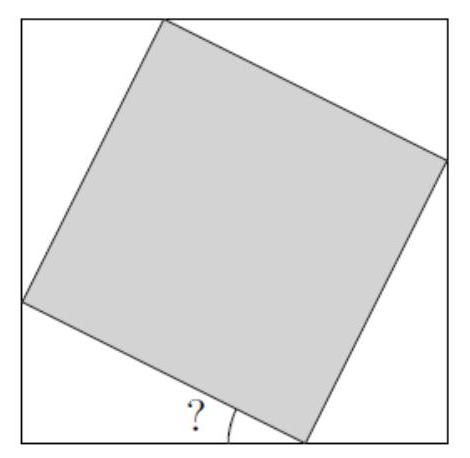
\includegraphics[max width=\textwidth, center]{2024_11_21_8c76d2422a3a02e654d7g-1}\\
3. Okrąg \(\omega_{3}\) o promieniu 3 jest styczny wewnętrznie do okręgów \(\omega_{1} \mathrm{i} \omega_{2}\) o promieniach odpowiednio 1 i 2. Co więcej, okręgi \(\omega_{1}\) i \(\omega_{2}\) są styczne zewnętrznie. Na okręgu \(\omega_{3}\) wybrano punkty A, B w taki sposób, że prosta AB jest wspólną styczną zewnętrzną okręgów \(\omega_{1} \mathrm{i} \omega_{2}\). Znajdź długość odcinka AB.


\end{document}